\documentclass[11pt]{article}
\usepackage[a4paper, margin=2.5cm]{geometry}
\usepackage{graphicx}
\usepackage{amsmath}
\usepackage{booktabs}
\usepackage{listings}
\usepackage{xcolor}
\usepackage[colorlinks=true, urlcolor=blue]{hyperref}
\usepackage{parskip}
\usepackage{float}

\lstset{
  basicstyle=\ttfamily\small,
  breaklines=true,
  frame=single,
  columns=fullflexible,
  showstringspaces=false,
  keepspaces=true,
}

% Visible placeholder box for a figure still to be drawn/inserted.
% Usage: \diagramplaceholder{caption text}
\newcommand{\diagramplaceholder}[1]{%
  \begin{center}
  \fbox{\parbox[c][3.2cm][c]{0.85\textwidth}{\centering\emph{#1}}}
  \end{center}}

% Framed note. Usage: \note{text}
\newcommand{\note}[1]{%
  \begin{center}
  \fbox{\parbox{0.94\textwidth}{\textbf{Note.} #1}}
  \end{center}}

\setcounter{tocdepth}{2}

\title{\textbf{PLSPS 2026 Assignment} \\ \textbf{Parallelising a Lattice Boltzmann Fluid Simulation}}
\author{Mikhail Cassar and Francesc Verdugo}
\date{2026}

\begin{document}

\begin{figure}[t]
\centering

\includegraphics[width=\textwidth]{diagrams/vua.png}
\end{figure}

\maketitle
\tableofcontents
\newpage

\section{Overview}

This document describes the PLSPS 2026 assignment. It outlines the problem, the required
parallelisation approach, the tasks, the grading scheme, and the deliverables. See the
\texttt{README.md} file for setup instructions and the commands to run, test, and benchmark the
code.

\textbf{You work on this assignment in pairs.} Form your group following in the instructions of the Canvas page for the assignment. All submissions are per group.

\subsection*{What you build}

The project provides a complete, working sequential fluid simulation written in Julia. You must
write a parallel solver, \texttt{run\_par}, that uses the Message Passing Interface (MPI) to
distribute the computation across several processes and produce the same result. After building the
solver, you must measure its parallel performance and report your findings.

\note{Your group only writes one file: \texttt{src/run\_par.jl}. Do not modify the \texttt{GeoFluidLBM.jl} file  or the sequential solver (\texttt{run\_seq}). You do not need to understand fluid dynamics to
complete this assignment.}

\subsection*{Grading}

Each objective corresponds to one of the four tasks in Section~\ref{sec:tasks}. The following table
lists the weight of each objective and the evidence we mark it against:

\begin{table}[H]
\centering
\begin{tabular}{@{}p{0.20\textwidth}p{0.55\textwidth}p{0.13\textwidth}@{}}
\toprule
Objective & Evidence & Weight \\
\midrule
\textbf{Implementation} & \texttt{run\_par.jl}, Report section 1 & 35\% \\
\textbf{Verification}   & \texttt{PASS} at 2 and 4 ranks on DAS-5, Report section 2 & Required \\
\textbf{Benchmarking}   & Report section 3 & 35\% \\
\textbf{Analysis}       & Report section 4 and 5 & 30\% \\
%\textbf{Presentation}   & Report & 10\% \\
\bottomrule
\end{tabular}
\end{table}

\textbf{Implementation:} We grade how well you describe the following aspects of the implementation: domain decomposition and work mapping, ghost column exchange, boundary conditions, and gathering the final result.

\textbf{Verification:} Your implementation must pass the provided tests at 2 and 4 ranks.
After the deadline we re-run these tests on DAS-5 with your submitted
\texttt{run\_par.jl}; our run is the one that counts. If either fails, you score 0\%
for Implementation. Other objectives are unaffected.

\textbf{Benchmarking:} We grade the parallel performance of your code and how well you describe the experimental setup and the quality of the figures showing your results. To assess the parallel performance, we will compare the parallel speedup of your code against the teacher's implementation. The teacher implementation obtains parallel speedup close to  the linear speedup for several (but not for all) of the test cases described below. If you never approach the linear speedup, there is something wrong with the parallel performance of your code.


\textbf{Analysis:} You should provide explanations for the effect of the grid size. For the cases that the speedup is significantly lower than the linear speedup, provide explanations about why this happens. In both cases, your explanations should combine hard evidence (e.g., computing communication over computation rations) and be supported by the theory studied in the course.

\note{Use the \LaTeX{} template provided in the folder \texttt{report} to write your report. Follow the structure given in the template. }

\textbf{Assignment grade:} The objective weights give a score out of 100\%. Your
assignment grade is $A = 1 + 9 \times (\text{score}/100)$, so a submitted assignment
is never graded below 1.




\subsection*{Reference material}

This assignment adapts a concise Python implementation of the lattice Boltzmann method by Mora,
Morra, and Yuen (2020)\footnote{\url{https://academic.oup.com/gji/article/220/1/682/5574400}}. We
recommend reading Section 5 of their paper. It clearly explains the decomposition, the neighbour
communication, and the gathering of results. \textbf{Reading the paper might be useful, but it is completely optional.} 

Because the paper's code is written in Python, its structure differs from the provided Julia
solver. Use the paper as a guide for the parallelisation approach rather than a template to copy.

\section{The simulation}

The lattice Boltzmann method (LBM) is a computational fluid dynamics technique. LBM simulates fluid
flow by tracking particle distribution functions on a fixed grid, rather than by solving the
Navier--Stokes equations directly.

\subsection*{The scenario}

The provided solver simulates pressure-driven channel flow, also known as Poiseuille flow. The
domain is a two-dimensional channel with solid walls on the top and bottom rows.

The solver drives the flow by holding the inlet (left) column at a higher density than the outlet
(right) column. The resulting pressure difference pushes fluid along the channel. At steady state,
the fluid moves fastest in the centre and stops at the walls. The velocity profile across the
channel forms an analytical parabola.

Figure~\ref{fig:flow} shows the flow field at steady state:

\begin{figure}[ht!]
    \centering
    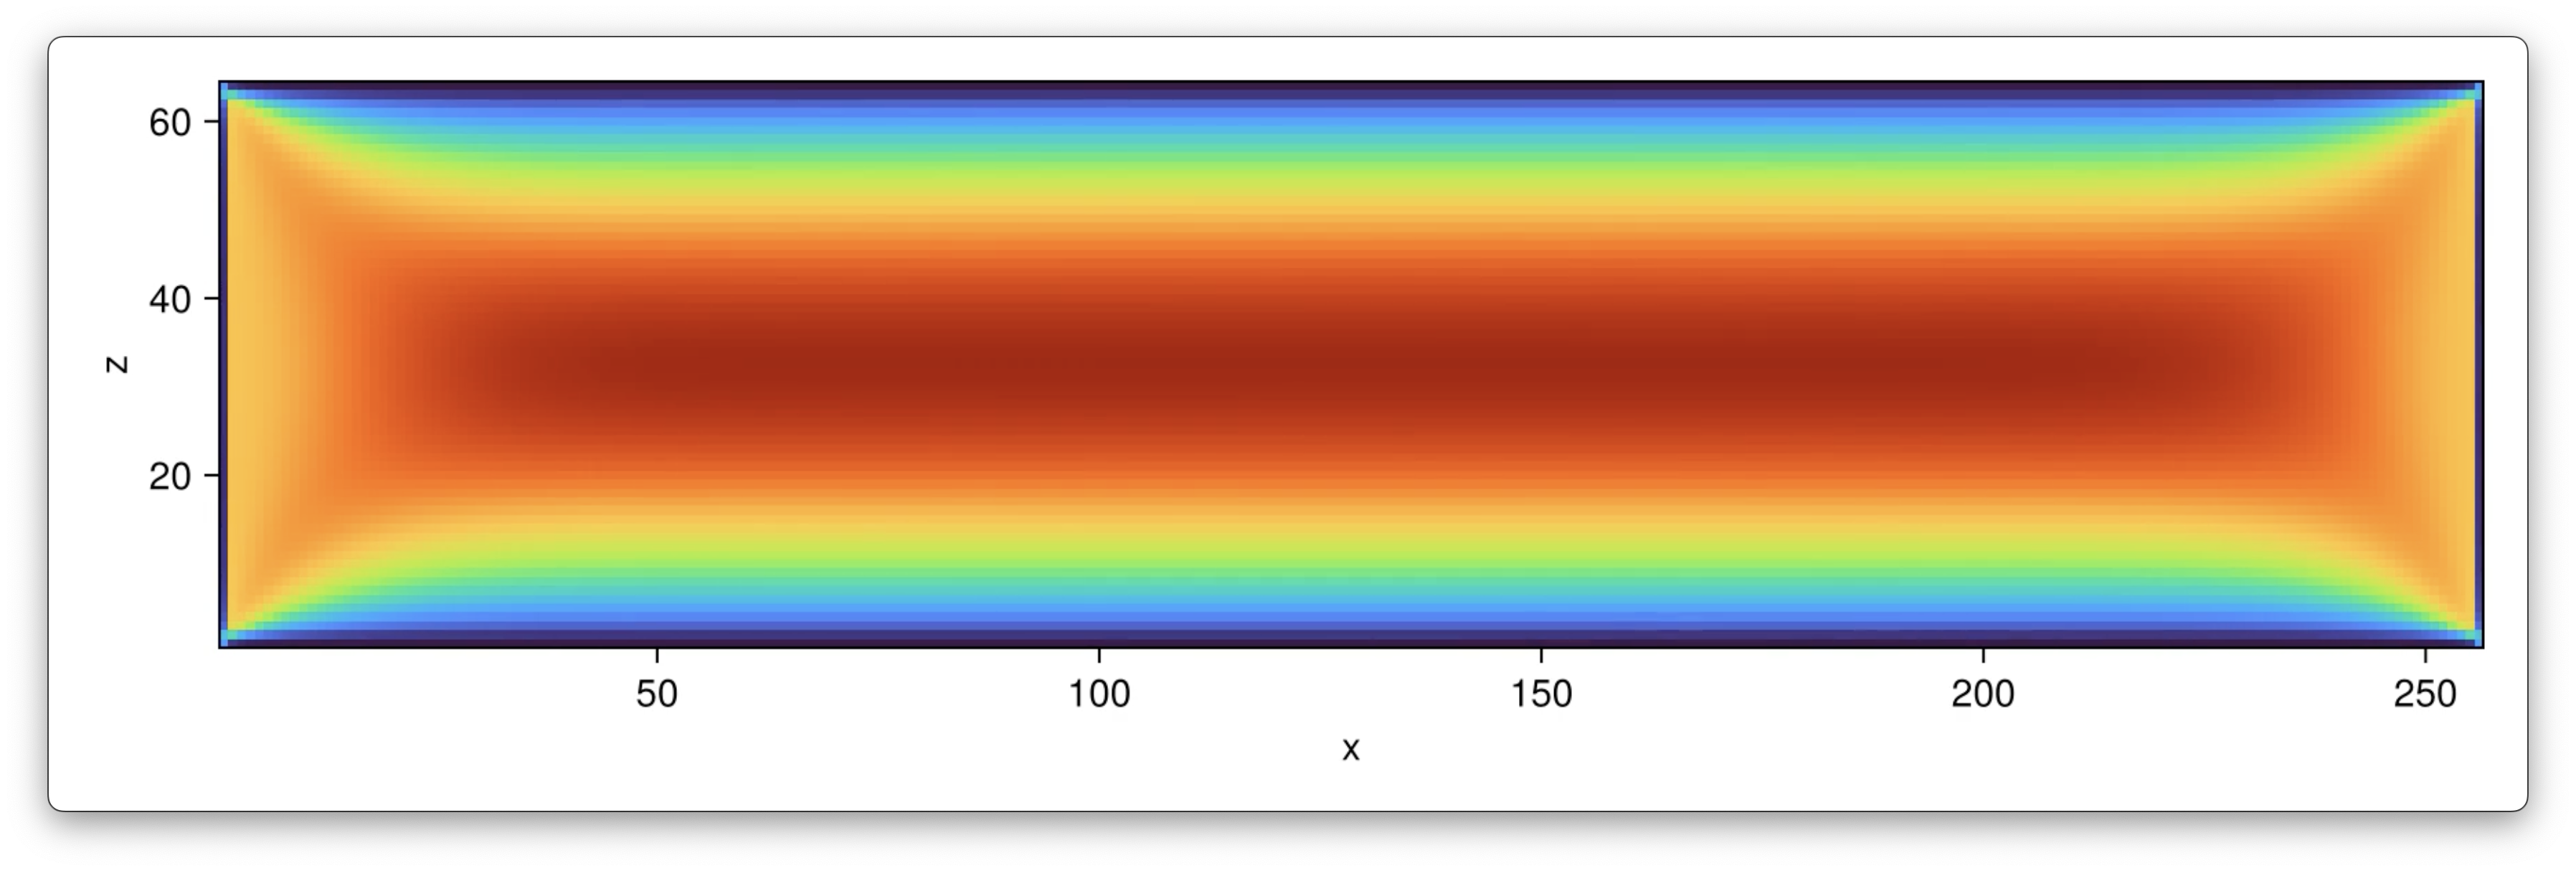
\includegraphics[width=0.5\linewidth]{diagrams/Poiseuille.png}
    \caption{Poiseuille flow.}
    \label{fig:flow}
\end{figure}

\subsection*{The lattice}

The solver discretises the two-dimensional domain into a uniform grid of cells called a
\textbf{lattice}. Lattice models use \textbf{D$n$Q$m$} notation, where $n$ is the number of spatial
dimensions and $m$ is the number of discrete velocities.

This solver uses the \textbf{D2Q9} model, so each cell holds 9 discrete velocity directions:

\begin{itemize}
  \item One direction for particles at rest.
  \item Four directions for the orthogonal axes: up, down, left, and right.
  \item Four directions for the diagonals.
\end{itemize}

Each cell therefore stores 9 particle distribution functions, $f_1 \dots f_9$, one per direction.
Figure~\ref{fig:d2qn} shows the nine directions:

\begin{figure}[ht!]
    \centering
    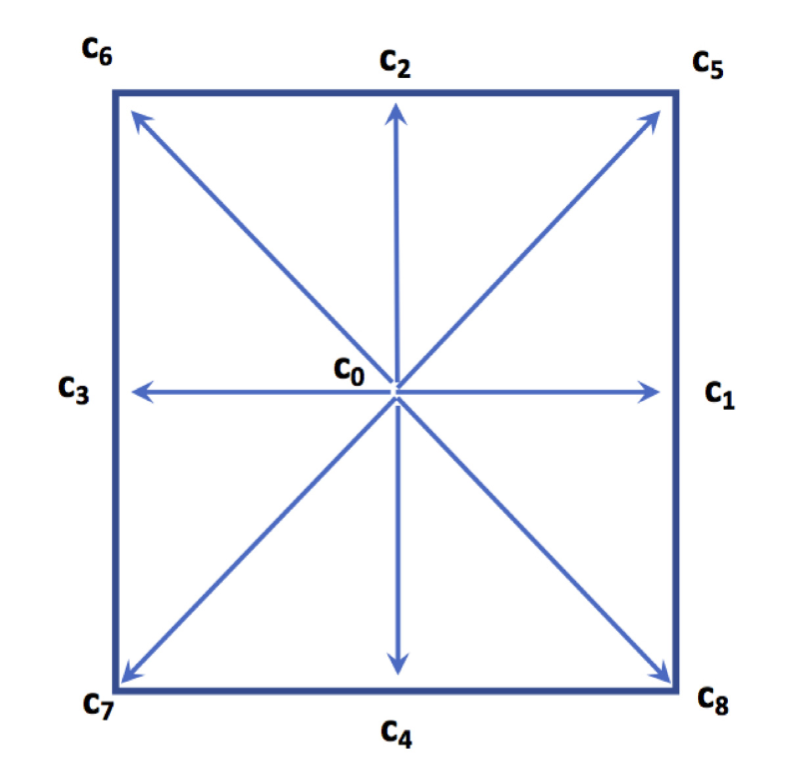
\includegraphics[width=0.4\linewidth]{diagrams/d2qn.png}
    \caption{\href{https://academic.oup.com/gji/article/220/1/682/5574400}{The D2Q9 lattice.}}
    \label{fig:d2qn}
\end{figure}

\subsection*{The sequential algorithm}

The project provides the sequential solver in \texttt{src/run\_seq.jl}. The solver evolves the
fluid in time by repeating a single timestep for $n_t$ steps. Each timestep runs the following four
steps in order:

\begin{enumerate}
  \item The \textbf{boundary step} drives the channel flow along $x$. It holds the leftmost column
        at density \texttt{rho\_in} and the rightmost column at the lower density
        \texttt{rho\_out}, by calling the helper \texttt{hold\_density!(s, x, rho)} once for each
        of the two columns. The step is written inline in \texttt{run\_seq}; \texttt{hold\_density!(s, x, rho)}
        lives in \texttt{GeoFluidLBM.jl} and is available to your parallel solver.
  \item \texttt{stream!} moves each particle distribution $f_i$ to the neighbouring cell in
        direction $i$. If the upstream cell is a solid wall, the particles bounce back. Streaming
        is the only step that reads data from neighbouring cells, and it reaches exactly one cell
        in each direction.
  \item \texttt{macroscopic!} recomputes the macroscopic fields from the current particle
        distributions \texttt{f}. The fields are the density \texttt{rho}, the momentum density
        \texttt{Pi}, and the velocity \texttt{u = Pi / rho}.
  \item \texttt{equilibrium\_collide!} performs the Bhatnagar--Gross--Krook (BGK) collision step.
        The function builds the local equilibrium \texttt{f\_eq} from \texttt{rho} and \texttt{u},
        then relaxes \texttt{f} towards it using
        $f \leftarrow f + (f_{\mathrm{eq}} - f)/\tau_f$. The collision step uses only local data.
\end{enumerate}

\subsection*{Data layout}

The solver stores particle distributions as \texttt{f[direction, z, x]} with shape
$(9, n_z, n_x)$:

\begin{itemize}
  \item $z$ is the vertical axis, which indexes rows.
  \item $x$ is the horizontal axis, which indexes columns.
\end{itemize}

Julia stores arrays in column-major order, so the first index varies fastest and the last index
varies slowest. Because $x$ is the last index, the slice \texttt{f[:, :, x]} occupies one contiguous
block of memory. That block holds an entire grid column.

\section{Parallelisation approach}
\label{sec:parallel}

\textbf{You must use a one-dimensional domain decomposition along $x$.} The decomposition splits
the grid into vertical strips of columns and assigns one strip to each MPI process. MPI identifies
each process by its \textbf{rank}, an integer from $0$ to $P - 1$, where $P$ is the total number of
processes. Each rank keeps the full grid height $n_z$.

You may assume that $n_x$ is a multiple of the number of MPI processes $P$. Your implementation does not need to handle a leftover strip of columns. Every grid used by the test and by the benchmark sweep has a power-of-two $n_x$, and every rank count is a power of two, so this assumption always holds.

Your implementation must perform the following:

\begin{itemize}
  \item \textbf{Exchange column data}: Exchange data between ``neighbouring'' ranks on every timestep
        to support cell streaming.
  \item \textbf{Apply boundary driving}: Apply the inlet and outlet driving only at the absolute
        ends of the global grid, not at the edges of individual strips.
  \item \textbf{Reconstruct the field}: Gather the final, full field on Rank 0 at the end of the
        run.
\end{itemize}

Further implementation details are found in Section 5 of the reference paper by Mora, Morra,
and Yuen (2020). That section explains the decomposition, neighbour communication, and gather
operations. \textbf{You may skip the paper completely and follow your own approach as long as it is based on a one-dimensional domain decomposition along the $x$ direction.}

\note{
In the paper, the calculations are
performed only on the secondary ranks, while the main rank sends and receives data, and creates output files. \textbf{We highly recommend to not follow this approach and assign a subdomain to all ranks including the main rank.} In this way, you get potentially better load balance and there is no need to handle a leftover strip of columns.

}

\note{
When implementing the neighbor exchange, it is highly recommended to pre-allocate the MPI request objects with function \texttt{MPI.Request} at the start of the simulation, before starting the time steps. Then, you can reuse these request objects at each time step, when calling  \texttt{MPI.Isend} and \texttt{MPI.Irecv!}. This is potentially faster than creating new request objects at each time step. See the documentation of these functions for further details. 
}

\section{Tasks}
\label{sec:tasks}

Complete the following four tasks.

\subsection*{Implement}

Implement \texttt{run\_par(cfg, comm)} in \texttt{src/run\_par.jl} by following the approach
detailed in Section~\ref{sec:parallel}. Your solver must meet the following two requirements:

\begin{itemize}
  \item \textbf{Match the sequential contract}: Rank 0 should return \texttt{(timings::Dict, state::State)}, matching the output of \texttt{run\_seq}. Ensure that Rank 0 holds the full gathered field
        within the \texttt{state} variable.
  \item \textbf{Record communication time}: Include a \texttt{"comm"} entry in the \texttt{timings}
        dictionary to store the time the solver spends communicating. Calculate the compute time
        using the formula: $\mathrm{compute} = \mathrm{total} - \mathrm{comm}$.
\end{itemize}

Answer the required questions and describe your implementation in Section 1 of the report template.

\subsection*{Verify}

The project provides a test that validates the following two conditions:

\begin{itemize}
  \item Both solvers reproduce the analytical Poiseuille parabola.
  \item The \texttt{run\_par} solver matches the \texttt{run\_seq} solver to round-off precision.
\end{itemize}

\note{The test must print \texttt{PASS} when running on both 2 ranks and 4 ranks. Passing on only 2
ranks is insufficient because it only exercises edge ranks, missing the interior case.}

Run the test on DAS-5. See the \texttt{README.md} for the commands. Report the verification outcome
in Section 2 of the report template.

\subsection*{Benchmark}

Run the strong-scaling benchmark on the DAS-5 cluster using the provided job script
\texttt{benchmark/\allowbreak benchmark\_job.sh}. The script sweeps each grid over $P \in \{1, 2, 4, 8, 16\}$ ranks for the three grid sizes listed in table~\ref{tab:grids}. Each run writes one JSON
record to \texttt{benchmark/results/}.% Because DAS-5 nodes have 16 physical cores\footnote{\url{https://www.cs.vu.nl/das5/clusters.shtml}}, runs up to $P = 16$ use a single node, while runs of $P = 32$ use two nodes.
%The following table lists the three fixed problem sizes for the strong-scaling benchmark:

\begin{table}[H]
\centering
\begin{tabular}{@{}lccc@{}}
\toprule
Grid   & $n_x$ & $n_z$ & $n_t$ \\
\midrule
Small  & 256   & 256   & 50 \\
Medium & 512   & 512   & 50 \\
Large  & 1024  & 1024  & 50 \\
\bottomrule
\end{tabular}
\caption{Fixed problem sizes for the strong-scaling benchmark.}
\label{tab:grids}
\end{table}

\note{Do not change the problem sizes. Each grid must remain constant as $P$ grows.}

Describe your experimental setup and present your measurements in Section 3 of the report template.

\subsection*{Analysis}

Extract all timing values from the \texttt{timings} dictionary within the JSON records. (Note: The
benchmark script automatically retains the fastest time from three repeated runs). Use the $P = 1$
record as your sequential baseline ($T_1$) for each grid.

The table~\ref{tab:metrics} lists the metrics you must compute for every grid and rank count:

\begin{table}[H]
\centering
\begin{tabular}{@{}lll@{}}
\toprule
Metric & Definition & Source \\
\midrule
Runtime $T_P$          & measured directly                & \texttt{timings["total"]} \\
Speedup $S(P)$         & $T_1 / T_P$                      & computed \\
Efficiency $E(P)$      & $S(P) / P$                       & computed \\
Communication fraction & $\mathrm{comm} / \mathrm{total}$ & computed \\
\bottomrule
\end{tabular}
\caption{Required metrics, per grid and rank count.}
\label{tab:metrics}
\end{table}

Present the completed tables and figures in Section 3 of the report template, which specifies their
required format. Answer the analysis questions in Sections 4 and 5.

\section{Submission}
\label{sec:submission}

Submit one \texttt{.zip} file per group to Canvas. Name the file
\texttt{PLSPS\_group\_[NUMBER].zip}.

\textbf{Deadline: Thursday October 22nd, 21:00.}

\note{Automatic scripts check every submission, so follow these instructions exactly.}

\subsection*{Required files}

Create a folder called  \texttt{PLSPS\_group\_[NUMBER]} and place exactly the following two files inside the folder. 

\begin{itemize}
  \item \textbf{Parallel implementation}: \texttt{run\_par.jl}
  \item \textbf{Report}: \texttt{Report\_group\_[NUMBER].pdf}
\end{itemize}

Then, compress the folder into a \texttt{.zip} file. Upload this \texttt{.zip} file to Canvas.

\subsection*{Rules}

The following rules apply to your submission:

\begin{itemize}
  \item \textbf{Report}: Follow the provided template. Limit the document to 5 pages,
        including tables and figures.
  \item \textbf{Implementation}: Build the solver with the Julia \texttt{MPI} package. Ensure it
        runs on DAS-5 with the provided job scripts without modification.
  \item \textbf{Groups}: As stated in the Overview, you work in pairs. Form your group on the Canvas groups page before submitting, as described on the course page.
  \item \textbf{Resubmission}: You may resubmit before the deadline. We mark only the last
        submission.
  \item \textbf{Late submissions}: We do not accept late submissions.
  \item \textbf{AI tools}: \textbf{Using AI is not needed at all to complete the assignment.} The less you use AI, the more you will practice and learn. You are allowed to use AI tools if you wish to assist you with the implementation, the formatting of figures and tables, and the proofreading of the report (fixing typos and enhancing phrasing and formatting). \textbf{It is strictly forbidden to run AI tools on DAS-5.} The results you present in the report must be based on the data you obtained on DAS-5 by running your own code. You remain fully accountable for everything you submit and must be able to explain all aspects of your work to the teachers. \textbf{Disclose any AI tool usage and its purpose in your report}. 
\end{itemize}

\textbf{Submissions that do not follow these instructions may receive a penalty.}

\subsection*{Anti-plagiarism rules}

All forms of plagiarism are strictly prohibited. These include, but are not limited to:
\begin{itemize}
\item using code from the Internet
\item making code publicly available on the Internet (e.g., on github)
\item using code from fellow students,
\item sharing code with fellow students
\item using code from former students
\item using AI beyond what is allowed in ``AI tools'' item above.
\end{itemize}



\section{Contact}
Ask questions on the Canvas discussion page. This is the main contact channel: post
there so the whole class benefits from the answer, and check it before posting in case
your question is already answered.

For private matters only, email one of the teaching assistants:
\begin{itemize}
  \item Olin Feist\\
        (\href{mailto:o.v.s.feist@student.vu.nl}{\texttt{o.v.s.feist@student.vu.nl}})
  \item Gabriel Gil Pichelbauer\\
        (\href{mailto:g.j.gilyanez@student.vu.nl}{\texttt{g.j.gilyanez@student.vu.nl}})
  \item Mahesh Karigoudar\\
        (\href{mailto:m.karigoudar@student.vu.nl}{\texttt{m.karigoudar@student.vu.nl}})
  \item Maria Couceiro Feio De Almeida Penalva\\
        (\href{mailto:m.couceirofeiodealmeidapenalva@student.vu.nl}%
        {\texttt{m.couceirofeiodealmeidapenalva@student.vu.nl}})
\end{itemize}

\end{document}
